\documentclass[../main/main]{subfiles}

\graphicspath{ {../assets/} }

\setcounter{chapter}{2} % one before

\begin{document}
    
\tableofcontents

\chapter[LQR]{Linear Quadratic Regulators}

\section{Motivation}

Have you ever tried balancing a pen upright on your palm?
If not, try it! It's a lot harder than seems.
Unlike the settings we studied in the previous chapter,
the state space and action space in this example aren'\hi \emph{finite}, or even \emph{discrete}.
Instead, they are \emph{continuous} (real-valued) and therefore \emph{uncountably infinite.}
In addition, the state transitions governing the system -- that is, the laws of physics --
are highly complex.

This task is an example of a classic \emph{control problem:}

\begin{figure}[h]
    \centering
    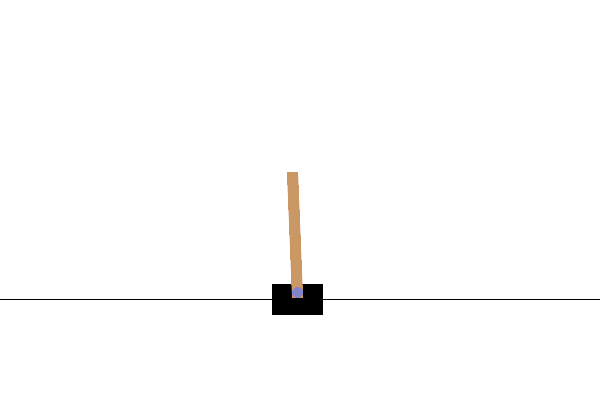
\includegraphics[width=0.5\textwidth]{cart_pole.png}
    \caption{CartPole: A pole balanced on a cart.}
    \label{fig:cart_pole}
\end{figure}

\begin{example}{CartPole}{cart_pole}
    Consider a pole balanced on a cart.
    The state $\st$ consists of just four continuous values:

    \begin{enumerate}
        \item The position of the cart;
        \item The velocity of the cart;
        \item The angle of the pole;
        \item The angular velocity of the pole.
    \end{enumerate}

    We can \emph{control} the cart by applying a horizontal force $\act$.

    \textbf{Goal:} Stabilize the cart around an ideal state and action $(\st^\star, \act^\star)$.
\end{example}

\emph{Controls} are the analogue to \emph{actions} in MDPs. In control theory, the state and controls are typically denoted as
$x$ and $u$, but we'll stick with the $\st$ and $\act$ notation to highlight the
similarity with MDPs.

Beyond this simple scenario, there are many real-world examples that involve continuous control. Here are just a few:
Autonomous driving, controlling a robot's joints, and automated manufacturing.
How can we teach computers to solve these kinds of problems?

\begin{figure}[h]
    \centering
    \begin{subfigure}[b]{0.45\textwidth}
        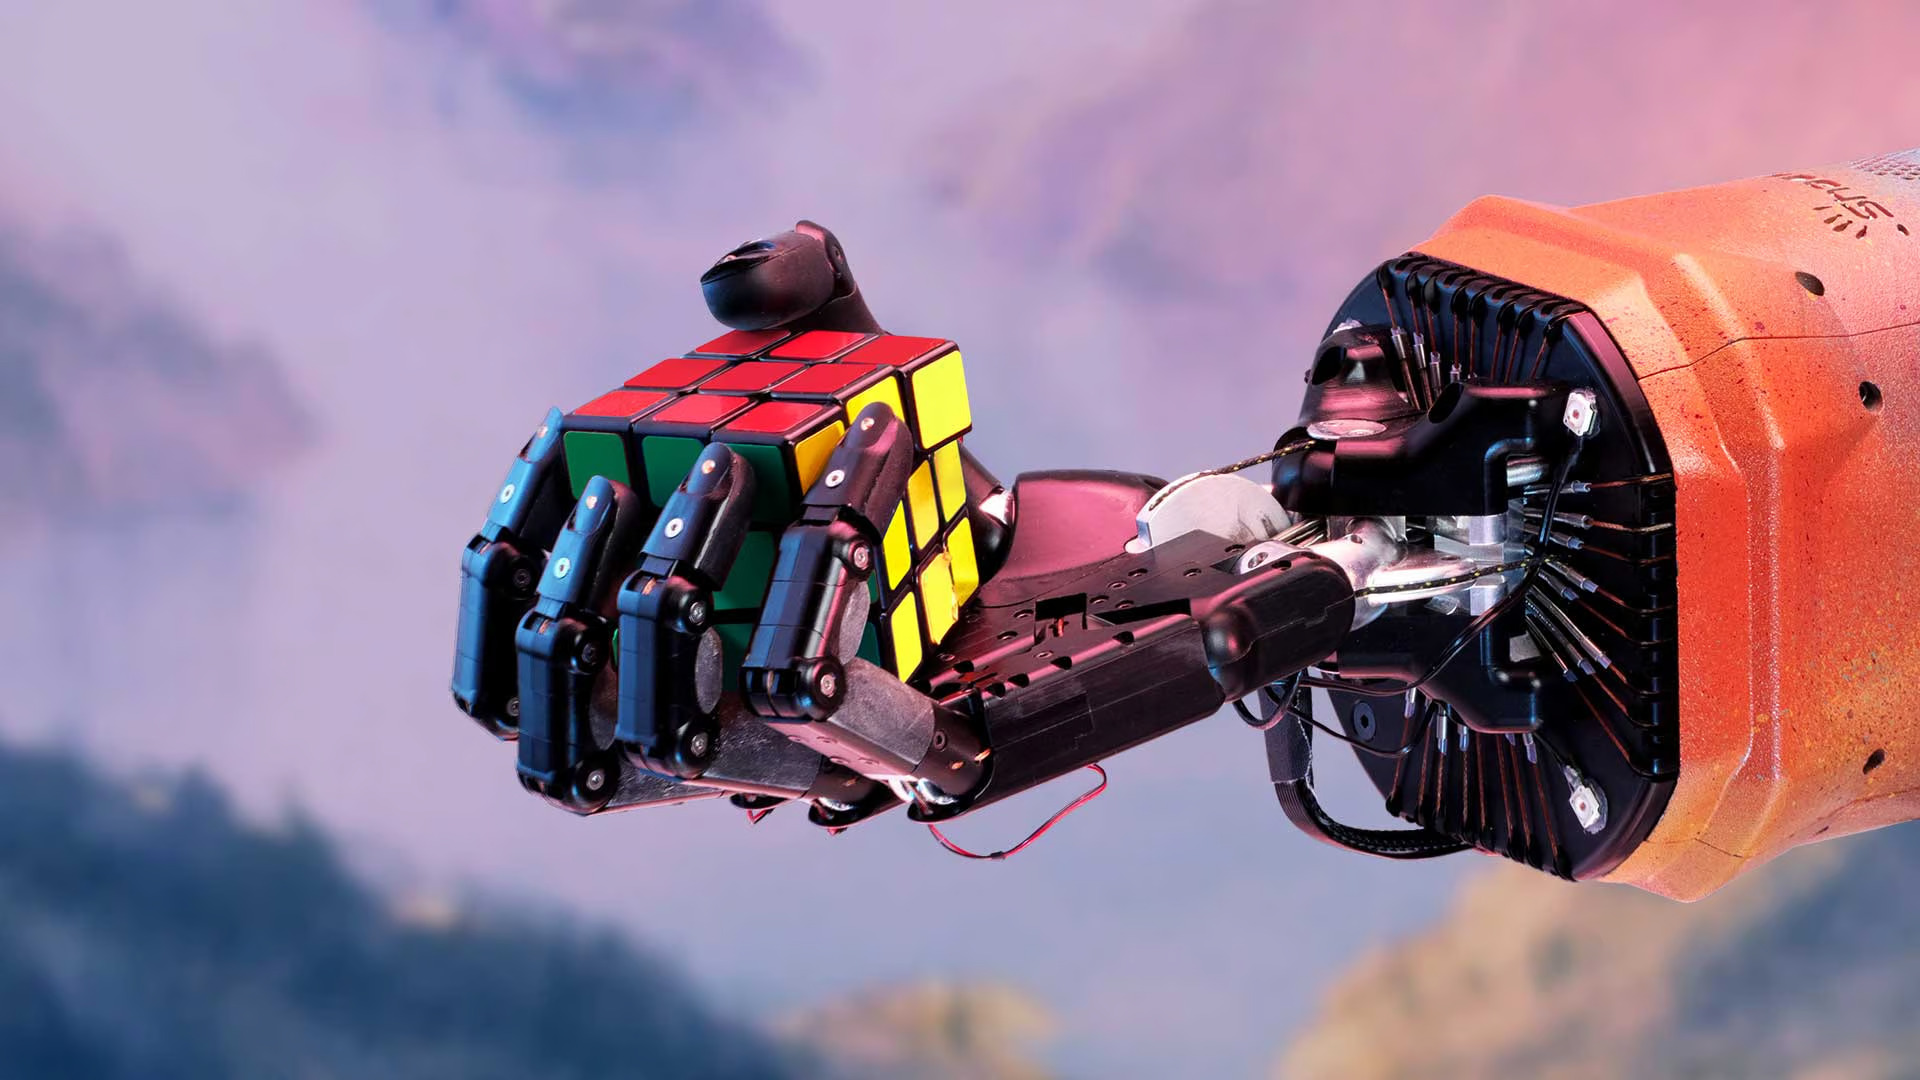
\includegraphics[width=\textwidth]{rubiks_cube.jpg}
        \caption{Solving a Rubik's Cube with a robot hand.}
        \label{fig:rubik\st_cube}
    \end{subfigure}
    \hfill
    \begin{subfigure}[b]{0.45\textwidth}
        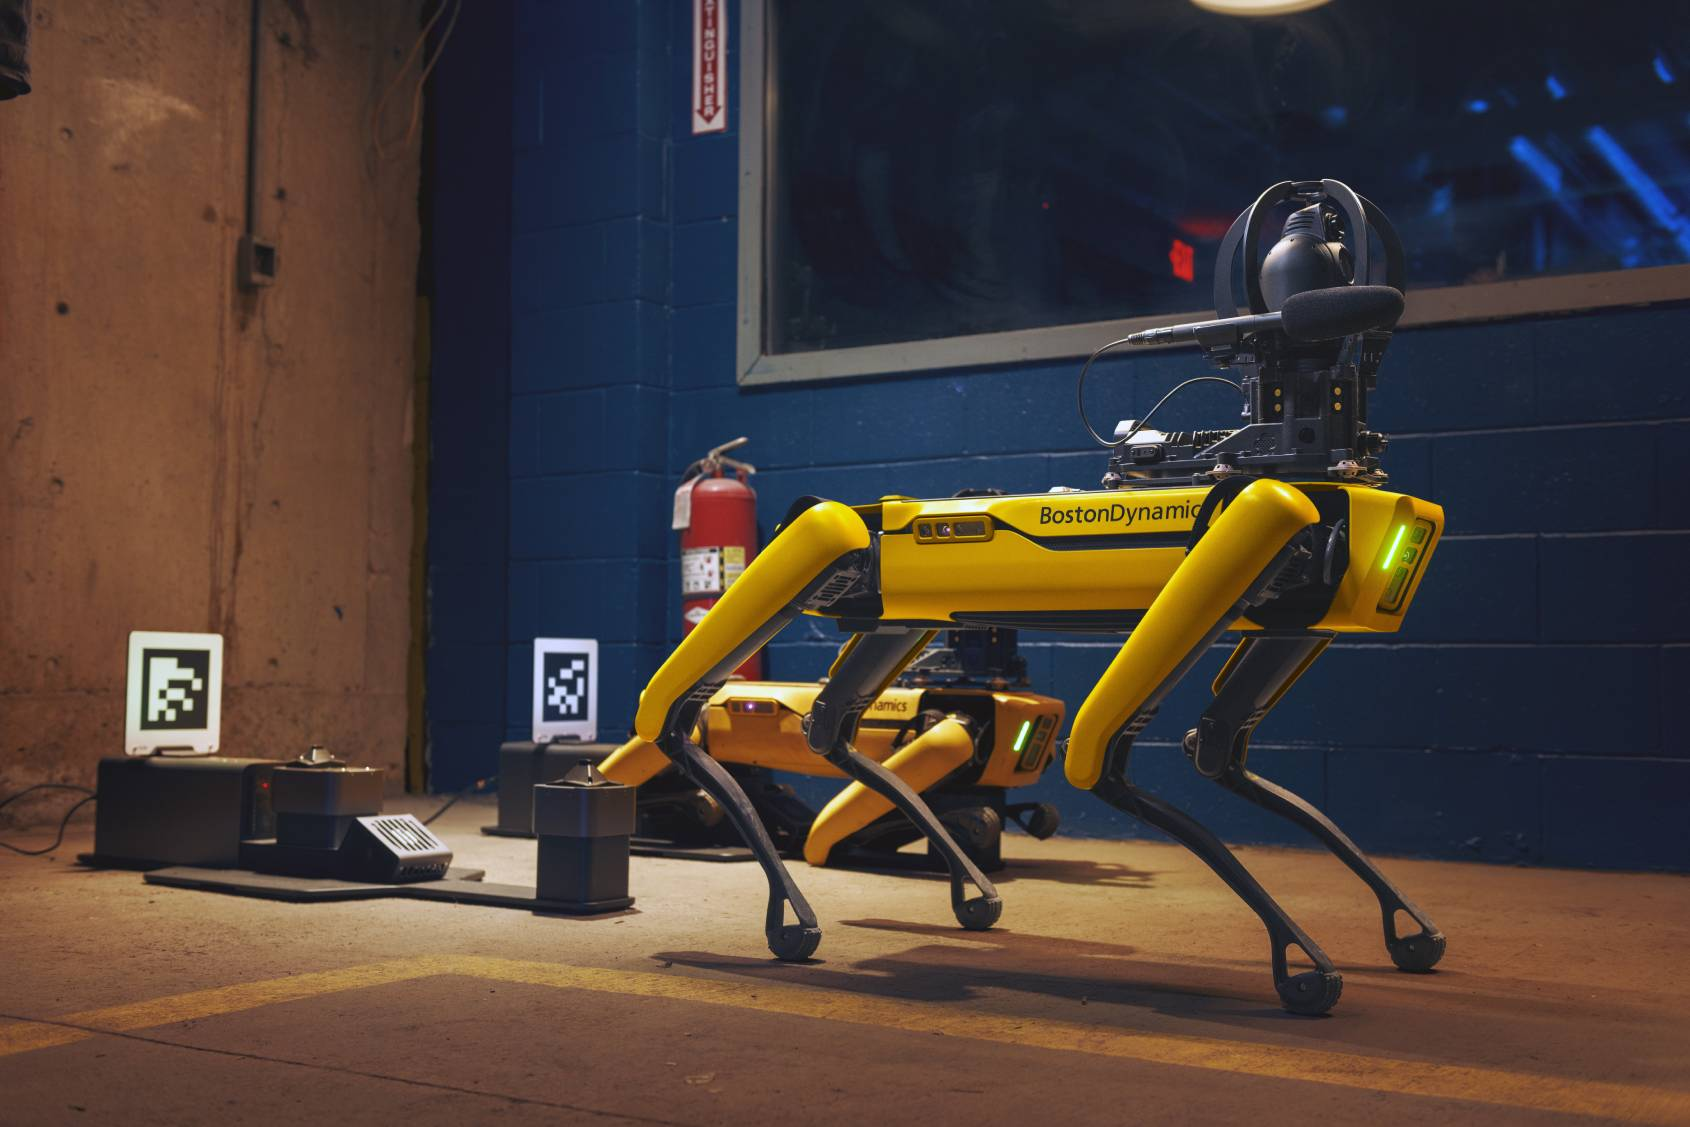
\includegraphics[width=\textwidth]{boston_dynamics.jpg}
        \caption{Boston Dynamics's Spot robot.}
        \label{fig:robot_hand}
    \end{subfigure}
    \caption{Examples of control tasks.}
    \label{fig:control_examples}
\end{figure}

In the last chapter, we developed efficient algorithms (\emph{value iteration} and \emph{policy iteration})
for calculating the optimal value function $V^\star$ and optimal policy $\pi^\star$ in an MDP.
In this chapter, we'll develop similar algorithms for the continuous control setting.

Note that we're still assuming that the entire environment is \emph{known} (i.e. the state transitions, rewards, etc). We'll explore the unknown case in the next chapter.

\section{Optimal control}

Recall that an MDP is defined by its state space $\S$, action space $\A$, state transitions $P$, reward function $r$, and discount factor $\gamma$ or time horizon $\hor$. What are the equivalents in the control setting?

\begin{itemize}
    \item The state and action spaces are \emph{continuous} rather than finite. That is, $\S = \R^{n_\st}$ and $\A = \R^{n_\act}$, where $n_\st$ and $n_\act$ are the number of coordinates to specify a single state or action respectively.
    \item We call the state transitions the \textbf{dynamics} of the system. In the most general case, these might change across timesteps and also include some stochastic \textbf{noise} $w_\hi$. We denote these dynamics as the function $f_\hi$, such that $\st_{\hi+1} = f_\hi(\st_\hi, \act_\hi, w_\hi)$. Of course, we can simplify to cases where the dynamics are \emph{deterministic/noise-free} (no $w_\hi$ term) or are \emph{stationary/time-homogeneous} (the same function $f$ across timesteps).
    \item Instead of a reward function, it's more common to consider a \textbf{cost function} $c_\hi: \S \times \A \to \R$ that describes \emph{how far away} we are from our \textbf{goal state-action pair} $(\st^\star, \act^\star)$. An important special case is when the cost is \emph{time-homogeneous}; that is, it remains the same function $c$ at each timestep.
    \item We seek to minimize the \emph{undiscounted} cost within a \emph{time horizon} $\hor$. Note that we end an episode at $\st_\hor$ -- there is no $\act_\hor$, and so we denote the cost for the final state as $c_\hor(\st_\hor)$.
\end{itemize}

With all of these components, we can now formulate the \textbf{optimal control problem:} \emph{find a time-dependent policy to minimize the expected undiscounted cost over $\hor$ timesteps.}

\begin{definition}{Optimal control problem}{optimal_control}
    \begin{equation}
        \begin{split}
            \min_{\pi_0, \dots, \pi_{\hor-1} : \S \to \A} \quad & \E_{\st_0, w_\hi} \left[
                \left( \sum_{\hi=0}^{\hor-1} c_\hi(\st_\hi, \act_\hi) \right) + c_\hor(\st_\hor)
            \right] \\
            \text{where} \quad & \st_{\hi+1} = f_\hi(\st_\hi, \act_\hi, w_\hi), \\
            & \act_\hi = \pi_\hi(\st_\hi) \\
            & \st_0 \sim \mu_0 \\
            & w_\hi \sim \text{noise}
        \end{split}
    \end{equation}
\end{definition}

% Note that this is a pretty hard problem the way it's written right now!
% We have some pretty strict constraints in the form of the state transitions.

\subsection{Discretization}

How does this relate to the finite horizon case?
If $\st_\hi$ and $\act_\hi$ were discrete, then we'd be able to work backwards using
the DP algorithms we saw before \eqref{df:pi_star_dp}.
% In this case, you can also think of $f_\hi$ as an (uncountably infinite-dimensional matrix.
A \st a matter of fact, let's consider what happens if we \emph{discretize} the
problem. For intuition, suppose $n_\st = n_\act = 1$ (that is, states and actions are real numbers).
To make $\S$ and $\A$ discrete, let's choose some small positive $\epsilon$,
and simply round states and actions to the nearest multiple of
$\epsilon$. For example, if $\epsilon = 0.01$, then we're just rounding $\st$ and $\act$ to two decimal spaces.
% \footnote{Formally, we can consider an $\epsilon$-net over the original continuous space. Let $V$ be some normed space. A subset $V_\epsilon \subseteq V$ is called an $\epsilon$-net if for all $v \in V$, there exists a $v_\epsilon \in V_\epsilon$ such that $\|v - v_\epsilon\| \le \epsilon$. The rounding example given is technically a $0.005$-net.} If both these state and action spaces can be bounded, then the resulting sets are actually finite, so now we can use our previous tools for MDPs.

How well does this work? Even if our $\S$ and $\A$ are
finite, the existing algorithms might take unfeasibly long to complete.
Suppose our state and action spaces
are bounded by some constants $\max_{\st \in \S} \|\st\| \le B_\st$ and
$\max_{\act \in \A} \|\act\| \le B_\act$.
Then using our rounding method, we must divide \emph{each dimension} into intervals of length $\varepsilon$,
resulting in $(B_\st/\varepsilon)^{n_\st}$ and $(B_\act/\varepsilon)^{n_\act}$ total points.
To get a sense of how quickly this grows, let's consider $\varepsilon = 0.01, n_\st = n_\act = 10$. Then the number of elements in our transition matrix is $|\S|^2 |\A| = (100^{10})^2 (100^{10}) = 10^{60}$!
Try finding a computer that'll fit that in memory! (For reference, 32 GB of memory can store $10^9$ 32-bit floating point numbers.)

So as we've seen, discretizing the problem becomes impractical as soon as
the action and state spaces are even moderately high-dimensional.
How can we do better?

Note that by discretizing the state and action spaces, we implicitly assumed that rounding each state or action vector by some tiny amount $\varepsilon$
wouldn'\hi change the behavior much; namely, that the functions involved were relatively \emph{continuous}.
Can we use this continuous structure in other ways? This brings us to the topic of \textbf{Linear Quadratic Regulators,} a widely used and studied tool in control theory.

\section{The Linear Quadratic Regulator Problem} \label{sec:lqr}

The optimal control problem stated above seems very difficult to solve.
The cost function might not be convex, making optimization difficult,
and the state transitions might be very complex, making it difficult to satisfy the constraints.
Is there a relevant simplification that we can analyze?

We'll show that a natural structure to impose is \emph{linear dynamics} and a \emph{quadratic cost function} (in both arguments). This is called the \textbf{linear quadratic regulator} (LQR) model, and is a popular tool in control theory.
In fact, some people even design systems to be linear in order to use results from LQR!

Why are these assumptions useful? A \st we'll see later in the chapter, it lets us \emph{locally approximate} nonlinear dynamics and cost functions
using their \emph{Taylor approximations} (up to first and second order respectively).
We'll also find that even for more complex setups,
we can generalize the algorithms for LQR to get surprisingly good solutions.

\begin{definition}{The linear quadratic regulator}{lqr}
    \textbf{Linear, time-homogeneous dynamics}: \[
        \st_{\hi+1} = f(\st_\hi, \act_\hi, w_\hi) = A \st_\hi + B \act_\hi + w_\hi
    \]

    \noindent \textbf{Quadratic, time-homogeneous cost function}:
    % TODO Link to that video in the multivariable calculus series
    % \footnote{For some intuition into this expression, consider the simple case where $\act_\hi$ and $\st_\hi$ are scalars (and so are $Q$ and $R$), so $c(\st_\hi, \act_\hi) = Q \st_\hi^2 + R \act_\hi^2$.
    % If this notation is unfamiliar to you, we recommend \href{https://www.khanacademy.org/math/multivariable-calculus/applications-of-multivariable-derivatives/quadratic-approximations/v/expressing-a-quadratic-form-with-a-matrix}{this tutorial on quadratic forms} from Khan Academy!
    % }
    \[
        c(\st_\hi, \act_\hi) = \begin{cases}
            \st_\hi^\top Q \st_\hi + \act_\hi^\top R \act_\hi & \hi < \hor \\
            \st_\hor^\top Q \st_\hor & \hi = \hor
        \end{cases}
    \]
    We want $c$ to be a convex function (easy to optimize) in both $\st_\hi$ and $\act_\hi$, so we'll set $Q$ and $R$ to both be positive definite matrices. We can furthermore assume without loss of generality that they are both symmetric (see exercise below).

    Intuitively, the cost function punishes states and actions that are far away from the origin (i.e. both the state and action are zero vectors). More generally, we'll want to replace the origin with a \emph{goal} state and action $(\st^\star, \act^\star)$. This can easily be done by replacing $\st_\hi$ with $(\st_\hi - \st^\star)$ and $\act_\hi$ with $(\act_\hi - \act^\star)$ in the expression above.
    

    \noindent \textbf{Spherical Gaussian noise:} \[ w_\hi \sim \mathcal{N}(0, \sigma^2 I) \]

    \noindent Putting everything together, the optimization problem we want to solve is:
    \begin{align*}
        \min_{\pi_0, \dots, \pi_{\hor-1} : \S \to \A} \quad & \E \left[ \left( \sum_{\hi=0}^{\hor-1} \st_\hi^\top Q \st_\hi + \act_\hi^\top R \act_\hi \right) + \st_\hor^\top Q \st_\hor \right] \\
        \textrm{where} \quad & \st_{\hi+1} = A \st_\hi + B \act_\hi + w_\hi \\
        & \act_\hi = \pi_\hi (\st_\hi) \\
        & w_\hi \sim \mathcal{N}(0, \sigma^2 I) \\
        & \st_0 \sim \mu_0.
    \end{align*}
\end{definition}

\textbf{Exercise:} We've set $Q$ and $R$ to be positive definite and symmetric. Here we'll show that the symmetry condition can be imposed without loss of generality. Show that replacing $Q$ with $(Q + Q^\top) / 2$ (which is symmetric) yields the same cost function.

\iffalse
% TODO We went over this example in lecture, but I'm not sure where in the chapter to put it.
\begin{example}{Driving down a road}{road_lqr}
    Suppose we're driving down a road. At each time step, we can choose an
    action $\act_\hi$: either we accelerate and apply a force forward ($\act_\hi > 0$),
    or reverse and apply a force backward ($\act_\hi < 0$).
    Suppose we can choose an action every $\delta$ seconds, and that our car
    has mass $m$.

    Recall that Newtonian mechanics says that $\text{force} = \text{mass} \times \text{acceleration}$. We can write the acceleration as the change in velocity
    over time, and write the velocity as the change in position over time:

    \begin{align*}
        \text{acceleration}_\hi &= \frac{v_\hi - v_{\hi-1}}{\delta} \\
        v_\hi &= \frac{p_\hi - p_{\hi-1}}{\delta} \\
    \end{align*}

    How should we construct our state? We want to express everything in terms
    of these linear dynamics, and we also want our state to be Markov, so that
    we can apply dynamic programming like before.
    Then if we write our state as consisting of the position and velocity, then
    we can write

    \begin{align*}
        p_{\hi+1} &= p_\hi  + \delta v_\hi \\
        v_{\hi+1} &= v_\hi + \frac{\delta}{m} \act_\hi
    \end{align*}

    Writing everything out in matrix notation, we get: \[
        \st_{\hi+1} = \begin{bmatrix}
            1 & \delta \\
            0 & 1
        \end{bmatrix} \begin{bmatrix}
            p_\hi \\ v_\hi
        \end{bmatrix}
        +
        \begin{bmatrix}
            0 \\ \frac{\delta}{m}
        \end{bmatrix}
        \act_\hi
    \]
\end{example}
\fi


So how do we go about analyzing this system? A good first step might be to introduce \emph{value functions,} analogous to those in the previous chapter, to reason about the behavior of the system over the time horizon.

\begin{definition}{Value functions for LQR}{value_lqr}
    Given a policy $\mathbf{\pi} = (\pi_0, \dots, \pi_{\hor-1})$, we can define the
    value function $V^\pi_\hi : \S \to \R$ as
    \[
        \begin{split}
            V^\pi_\hi (\st) &= \E \left[ \left( \sum_{i=\hi}^{\hor-1} c(\st_i, \act_i) \right) + c(\st_\hor) \mid \st_\hi = \st,  \forall i \ge \hi. \act_i = \pi_i(\st_i) \right] \\
            &= \E \left[ \left( \sum_{i=\hi}^{\hor-1} \st_i^\top Q \st_i + \act_i^\top R \act_i \right) + \st_\hor^\top Q \st_\hor \mid \st_\hi = \st, \forall i \ge \hi. \act_i = \pi_i(\st_i) \right] \\
        \end{split}
        % old notation:
        % \begin{split}
        %     V^\pi_\hi (\st) &= \E \left[ \left( \sum_{i=\hi}^{\hor-1} c(\st_i, \act_i) \right) + c(\st_\hor) \right] \\
        %     &= \E \left[ \left( \sum_{i=\hi}^{\hor-1} \st_i^\top Q \st_i + \act_i^\top R \act_i \right) + \st_\hor^\top Q \st_\hor \right] \\
        %     \textrm{conditional on} \quad \st_\hi &= \st \\
        %     \act_i &= \pi_i(\st_i) \quad \forall i \ge \hi.
        % \end{split}
    \]
    The expression inside the expectation is called the \textbf{cost-to-go},
    since it's just the total cost starting from timestep $\hi$.

    The $Q$ function additionally conditions on the first
    action we take:
    \[
        \begin{split}
            Q^\pi_\hi (\st, \act) &= \E \left[ \left( \sum_{i=\hi}^{\hor-1} c(\st_i, \act_i) \right) + c(\st_\hor) \mid  (\st_\hi, \act_\hi) = (\st, \act), \forall i \ge \hi. \act_i = \pi_i(\st_i) \right] \\
            &= \E \left[ \left( \sum_{i=\hi}^{\hor-1} \st_i^\top Q \st_i + \act_i^\top R \act_i \right) + \st_\hor^\top Q \st_\hor \mid (\st_\hi, \act_\hi) = (\st, \act), \forall i \ge \hi. \act_i = \pi_i(\st_i) \right] \\
        \end{split}
        % \begin{split}
        %     Q^\pi_\hi (\st, \act) &= \E \left[ \left( \sum_{i=\hi}^{\hor-1} c(\st_i, \act_i) \right) + c(\st_\hor) \right] \\
        %     &= \E \left[ \left( \sum_{i=\hi}^{\hor-1} \st_i^\top Q \st_i + \act_i^\top R \act_i \right) + \st_\hor^\top Q \st_\hor \right] \\
        %     \textrm{conditional on} \quad (\st_\hi, \act_\hi) &= (\st, \act) \\
        %     \quad \act_i &= \pi_i(\st_i) \quad \forall i > \hi
        % \end{split}
    \]
\end{definition}

A \st in the previous chapter, these will be instrumental in constructing optimal policy $\pi$ via dynamic
programming.

\section{Optimality and the Riccati Equation} \label{sec:optimal_lqr}

In this section, we'll compute the optimal value function and policy in the LQR setting using \textbf{dynamic programming}, in a very similar way to the DP algorithms we saw in the previous chapter. % TODO add reference for completed version.
\begin{enumerate}
    \item We'll compute $V_H^\star(x)$ as our base case.
    \item Then we'll work backwards, using $V_{h+1}^\star(x)$ to compute $Q_h^\star(x, u)$, $\pi_{h+1}^\star(x)$, and $V_h^\star(x)$.
\end{enumerate}
Along the way, we will prove that $V_h^\star$ and $\pi_h^\star$ have very simple structure: $V_h^\star(x)$ is a \emph{convex quadratic} and $\pi_h^\star(x)$ is \emph{linear}.

\begin{definition}[breakable=false]{Optimal value functions for LQR}{optimal_value_lqr}
    The \textbf{optimal value function} is the one that, at any time, in any state,
    achieves \emph{minimum cost} across \emph{all policies}: \[
        \begin{split}
            V^\star_\hi(\st) &= \min_{\pi_\hi, \dots, \pi_{\hor-1}} V^\pi_\hi(\st) \\
            &= \min_{\pi_{\hi}, \dots, \pi_{\hor-1}} \E \left[ \left( \sum_{i=\hi}^{\hor-1} \st_\hi^\top Q \st_\hi + \act_\hi^\top R \act_\hi \right) + \st_\hor^\top Q \st_\hor
            \mid \st_\hi = \st, \act_i = \pi_i(\st_i) \quad \forall i \ge \hi \right] \\
        \end{split}
    \]
\end{definition}

\begin{theorem}{Optimal value function in LQR is a convex quadratic}{optimal_value_lqr_quadratic}
    \[
        V^\star_\hi(\st) = \st^\top P_\hi \st + p_\hi
    \]
    for some time-dependent $P_\hi \in \R^{n_\st \times n_\st}$ and $p_\hi \in \R^{n_\st}$ where $P_\hi$ is symmetric and positive definite. Note that there is no linear term.
\end{theorem}

\begin{theorem}{Optimal policy in LQR is linear}{optimal_policy_lqr_linear}
    \[
        \pi^\star_\hi (\st) = - K_\hi \st
    \]
    for some $K_\hi \in \R^{k \times d}$. (The negative is due to convention.)
\end{theorem}


% How can we define an optimal time-dependent policy in this setting?

% It turns out that the optimal policy is one that is deterministic and \emph{linear} at each time
% step! That is, \[ \pi_\hi^\star (\st_\hi) = - K_\hi \st_\hi. \] We'll prove this more
% formally in \autoref{th:optimal_policy_lqr_linear}. This should remind you somewhat of the way in which the optimal policy in
% the previous MDP setting was stationary and deterministic. In both cases,
% it turns out that the optimal policy has special structure!


\textbf{Base case:} $V^\star_\hor(\st) = \st^\top P_\hor \st + p_\hor$. At the final timestep, there are no possible actions to take, and so $V^\star_\hor(\st) = c(\st) = \st^\top Q \st$. Thus $P_\hor = Q$ and $p_\hor$ is the zero vector.

\textbf{Inductive hypothesis:} We seek to show that the inductive step holds for both theorems: If $V^\star_{\hi+1}(\st)$ is a convex quadratic, then $V^\star_\hi(\st)$ must also be a convex quadratic, and $\pi^\star_\hi(\st)$ must be linear. We'll break this down into the following steps:
\begin{steps}
    \item Show that $Q^\star_\hi(\st, \act)$ is a convex quadratic (in both $\st$ and $\act$).
    \item Derive the optimal policy $\pi^\star_\hi(\st) = \arg \min_\act Q^\star_\hi(\st, \act)$ and show that it's linear.
    \item Show that $V^\star_\hi(\st)$ is a convex quadratic.
\end{steps}
This is essentially the same proof that we wrote in the finite-horizon MDP setting,
except now the state and action are \emph{continuous} instead of finite.

We first assume our theorems are true at time $\hi+1$. That is,
\[ V^\star_{\hi+1}(\st) = \st^\top P_{\hi+1} \st + p_{\hi+1} \quad \text{for all states} \quad \st \in \S. \]

\textbf{Step 1.} We'll start off by demonstrating that $Q^\star_\hi(\st)$ is a convex quadratic.
Recall that the definition of $Q^\star_\hi : \S \times \A \to \R$ is \[
    Q^\star_\hi(\st, \act) = c(\st, \act) + \E_{\st' \sim f(\st, a, w_{\hi+1})} V^\star_{\hi+1}(\st').
\]
We know $c(\st, \act) := \st^\top Q \st + \act^\top R \act$. Let's consider the average value
over the next timestep. The only randomness in the dynamics comes from the noise
$w_{\hi+1}$, so we can write out this expected value as:
\begin{align*}
    &\qquad \E_{\st' \sim f(\st, a, w_{\hi+1})} V^\star_{\hi+1}(\st') \\
    &= \E_{w_{\hi+1} \sim \cN(0, \sigma^2 I)} V^\star_{\hi+1}(A \st + B \act + w_{\hi+1}) && \text{definition of } f \\
    &= \E_{w_{\hi+1}} [ (A \st + B \act + w_{\hi+1})^\top P_{\hi+1} (A \st + B \act + w_{\hi+1}) + p_{\hi+1} ]. && \text{inductive hypothesis}
\end{align*}
Summing and combining like terms, we get \begin{align*}
    Q^\star_\hi(\st, \act) &= \st^\top Q \st + \act^\top R \act + \E_{w_{\hi+1}} [(A \st + B \act + w_{\hi+1})^\top P_{\hi+1} (A \st + B \act + w_{\hi+1}) + p_{\hi+1}] \\
    &= \st^\top (Q + \act^\top P_{\hi+1} A)\st + \act^\top (R + B^\top P_{\hi+1} B) a + 2 \st^\top \act^\top P_{\hi+1} B a \\
    &\qquad + \E_{w_{\hi+1}} [w_{\hi+1}^\top P_{\hi+1} w_{\hi+1}] + p_{\hi+1}.
\end{align*}
Note that the terms that are linear in $w_\hi$ have mean zero and vanish.
Now consider the remaining expectation over the noise. By expanding out the product and using linearity of
expectation, we can write this out as \begin{align*}
    \E_{w_{\hi+1}} [w_{\hi+1}^\top P_{\hi+1} w_{\hi+1}] &= \sum_{i=1}^d \sum_{j=1}^d (P_{\hi+1})_{ij} \E_{w_{\hi+1}} [(w_{\hi+1})_i (w_{\hi+1})_j].
\end{align*}
When dealing with these \emph{quadratic forms}, it's often helpful to consider the terms
on the diagonal ($i = j$) separately from those off the diagonal. On the diagonal, the
expectation becomes \[ (P_{\hi+1})_{ii} \E (w_{\hi+1})_i^2 = (P_{\hi+1})_{ii} \var \big((w_{\hi+1})_i \big) = \sigma^2 (P_{\hi+1})_{ii}. \]
Off the diagonal, since the elements of $w_{\hi+1}$ are independent,
the expectation factors, and since each element has mean zero, the term disappears: \[ (P_{\hi+1})_{ij} \E (w_{\hi+1})_i \E (w_{\hi+1})_j = 0. \]
Thus, the only terms left are the ones on the diagonal, so the sum of these can
be expressed as the trace of $\sigma^2 P_{\hi+1}$: \[
    \E_{w_{\hi+1}} [w_{\hi+1}^\top P_{\hi+1} w_{\hi+1}] = \tr(\sigma^2 P_{\hi+1}).
\]
Substituting this back into the expression for $Q^\star_\hi$, we have:

\begin{equation}
    \boxed{
        \begin{aligned}
            Q^\star_\hi(\st, \act) &= \st^\top (Q + \act^\top P_{\hi+1} A) \st + \act^\top (R + B^\top P_{\hi+1} B) a
            + 2\st^\top \act^\top P_{\hi+1} B a \\
            &\qquad + \tr(\sigma^2 P_{\hi+1}) + p_{\hi+1}.
        \end{aligned}
    }
    \label{eq:q_star_lqr}
\end{equation}

A \st we hoped, this expression is quadratic in $\st$ and $\act$.
Furthermore, we'd like to show that it also has positive curvature with respect to $\act$ so that its minimum with respect to $\act$ is well-defined.
This is fairly straightforward:

\begin{theorem}{$Q^\star_\hi$ is a convex quadratic}{optimal_q_convex}
    Consider the part of \autoref{eq:q_star_lqr} that is quadratic in $\act$, namely
    $\act^\top (R + B^\top P_{\hi+1} B) \act$. Then $Q^\star_\hi$ is a convex quadratic with respect to $\act$
    if $R + B^\top P_{\hi+1} B$ is symmetric and positive definite (SPD).
\end{theorem}

To see why this is the case, recall that in our definition of LQR,
we assumed that $R$ is SPD (see \autoref{df:lqr}).
Also note that since $P_{\hi+1}$ is SPD (by the inductive hypothesis), so too must be $B^\top P_{\hi+1} B$. (If this isn'\hi clear, try proving it as an exercise!)
Since the sum of two SPD matrices is also SPD, we have that $R + B^\top P_{\hi+1} B$ is SPD,
and so $Q^\star_\hi$ is convex with respect to $\act$. A similar proof shows that $Q + \act^\top P_{\hi+1} A$ is SPD, and so $Q^\star_\hi$ is also a convex quadratic.

\textbf{Step 2.} Now let's move on to the next part of proving the inductive hypothesis:
showing that $\pi^\star_\hi(\st) = \arg \min_\act Q^\star_\hi(\st, \act)$ is linear.
Since $Q^\star_\hi$ is a convex quadratic, finding its minimum over $\act$ is easy:
we can just take the gradient with respect to $\act$ and set it to zero.
First, we calculate the gradient:
\begin{align*}
    \nabla_\act Q^\star_\hi(\st, \act) &= \nabla_\act [ \act^\top (R + B^\top P_{\hi+1} B) a + 2 \st^\top \act^\top P_{\hi+1} B a ] \\
    &= 2 (R + B^\top P_{\hi+1} B) a + (2 \st^\top \act^\top P_{\hi+1} B)^\top
\end{align*}
Setting this to zero, we get \begin{align}
    0 &= (R + B^\top P_{\hi+1} B) a + B^\top P_{\hi+1} A \st \nonumber \\
    \pi^\star_\hi(\st) := a &= -(R + B^\top P_{\hi+1} B)^{-1} B^\top P_{\hi+1} A \st \nonumber \\
    &= - K_\hi \st,
\end{align}
where $K_\hi = (R + B^\top P_{\hi+1} B)^{-1} B^\top P_{\hi+1} A$.

Note that this optimal policy has an interesting property: in addition to being
independent of the starting distribution $\mu_0$ (which also happened for our
finite-horizon MDP solution), it's also fully deterministic and isn'\hi affected by noise!
(Compare this with the discrete MDP case, where calculating our optimal policy
required taking an expectation over the state transitions.)

\textbf{Step 3.} To complete our inductive proof, we must show that the
inductive hypothesis is true at time $\hi$; that is, we must prove that
$V^\star_\hi(\st)$ is quadratic.
Using the identity $V^\star_\hi(\st) = Q^\star_\hi(\st, \pi^\star(\st))$, we have: \begin{align*}
    V^\star_\hi(\st) &= Q^\star_\hi(\st, \pi^\star(\st)) \\
    &= \st^\top (Q + \act^\top P_{\hi+1} A) \st + (-K_\hi \st)^\top (R + B^\top P_{\hi+1} B) (-K_\hi \st)
    + 2\st^\top \act^\top P_{\hi+1} B (-K_\hi \st) \\
        &\qquad + \tr(\sigma^2 P_{\hi+1}) + p_{\hi+1}
\end{align*}
Note that with respect to $\st$, this is the sum of a quadratic term and a constant,
which is exactly what we were aiming for!

To conclude our proof, let's concretely specify the values of $P_\hi$ and $p_\hi$.
The constant term is clearly $p_\hi = \tr(\sigma^2 P_{\hi+1}) + p_{\hi+1}$.
We can simplify the quadratic term by substituting in $K_\hi$.
Notice that when we do this, the $(R+B^\top P_{\hi+1} B)$ term in
the expression is cancelled out by its inverse, and the remaining terms combine to give
what is known as the \emph{Riccati equation:}

\begin{definition}{Riccati equation}{riccati}
    \[
        P_\hi = Q + \act^\top P_{\hi+1} A - \act^\top P_{\hi+1} B (R + B^\top P_{\hi+1} B)^{-1} B^\top P_{\hi+1} A.
    \]
\end{definition}

There are several nice things to note about the Riccati equation:
\begin{enumerate}
    \item It's defined \textbf{recursively.} Given the dynamics defined by $\act$ and $B$, and the state coefficients $Q$, we can
    recursively calculate $P_\hi$ across all timesteps starting from $P_\hor = Q$.
    \item $P_\hi$ often appears in calculations surrounding optimality, such as $V^\star_\hi, Q^\star_\hi$, and $\pi^\star_\hi$.
    \item Together with $A, B$, and the action coefficients $R$, it fully defines the optimal policy.
\end{enumerate}

Now we've shown that $V^\star_\hi(\st) = \st^\top P_\hi \st + p_\hi$, which is a convex quadratic, and this concludes our proof. \qed

In summary, we just demonstrated that:

\begin{itemize}
    \item The optimal value function $V^\star_\hi$ is convex at all $\hi$.
    \item The optimal $Q$-function $Q^\star_\hi$ is convex (in both arguments) at all $\hi$.
    \item The optimal policy $\pi^\star_\hi$ is linear at all $\hi$.
    \item All of these quantities can be calculated using a symmetric matrix $P_\hi$ for each timestep, which can be defined recursively using the Riccati equation.
\end{itemize}

Before we move on to some extensions of LQR, let's consider how the state at time $\hi$ behaves when we act according to this optimal policy.

\subsection{Expected state at time $\hi$}

% TODO would a finance example be better here? Probably not realistic

Suppose you're about to go to bed, and the thermostat in your room is controlled by an optimal policy under LQR. A very reasonable question to ask would be: what's the expected state (i.e. temperature) of the room at a given time $\hi$? Certainly you don'\hi want to freeze or boil overnight!

To answer this question, let's first express the state at time $\hi$ in a cleaner way in terms of the history. Note that having linear dynamics makes it easy to expand terms backwards in time:
\begin{align*}
    \st_\hi &= A \st_{\hi-1} + B \act_{\hi-1} + w_{\hi-1} \\
    &= A (A\st_{\hi-2} + B \act_{\hi-2} + w_{\hi-2}) + B \act_{\hi-1} + w_{\hi-1} \\
    &= \cdots \\
    &= \act^\hi \st_0 + \sum_{i=0}^{\hi-1} \act^i (B \act_{\hi-i-1} + w_{\hi-i-1}).
\end{align*}

Let's consider the \emph{average state} at this time, given all the past states and actions.
Since we assume that $\E w_\hi = 0$ (this is the zero vector in $d$ dimensions),
when we take an expectation, the $w_\hi$ term vanishes due to linearity, and so we're left with \[
    \E [\st_\hi \mid \st_{0:(\hi-1)}, \act_{0:(\hi-1)}] = \act^\hi \st_0 + \sum_{i=0}^{\hi-1} \act^i B \act_{\hi-i-1}.
\]
If we choose actions according to our optimal policy, this becomes \[
    \E [\st_\hi \mid \st_0, \forall i \le \hi . \act_i = - K_i \st_i] = \left( \prod_{i=0}^{\hi-1} (A - B K_i) \right) \st_0.
\]
This introdces the quantity $A - B K_i$, which shows up frequently in control theory.
For example, one important question is: will $\st_\hi$ remain bounded,
or will it go to infinity as time goes on?
To answer this, let's imagine that these $K_i$\st are equal (call this matrix $K$).
Then the expression above becomes $(A-BK)^\hi \st_0$.
Now consider the maximum eigenvalue $\lambda_{\max}$ of $A - BK$.
If $|\lambda_{\max}| > 1$, then there's some nonzero initial state $\bar \st_0$, the corresponding eigenvector, for which \[
    \lim_{\hi \to \infty} (A - BK)^\hi \bar \st_0 = \lambda_{\max}^\hi \bar \st_0 = \infty.
\]
By then, your room is \emph{definitely} on fire! Otherwise, if $|\lambda_{\max}| < 1$, then it's impossible for your original state to explode as dramatically (assuming it's properly normalized).

We've now formulated an optimal solution for the typical, time-homogeneous case of LQR, and considered the expected state under the optimal policy.
However, this simple case is insufficient for more complex tasks.
In the following sections, we'll consider some motivating examples, and extensions of LQR where some assumptions are relaxed.

\section{Extensions}

In this section, we'll consider settings where some of the assumptions we made above are relaxed.
Specifically, we'll consider:
\begin{enumerate}
    \item \textbf{Time-dependency,} where the dynamics and cost function might change depending on the timestep.
    \item \textbf{General quadratic cost,} where we allow for linear terms and a constant term.
    \item \textbf{Tracking a goal trajectory} rather than aiming for a single goal state-action pair.
\end{enumerate}

\subsection[Time-dependency]{Time-dependent dynamics and cost function} \label{sec:time_dep_lqr}

So far, we've considered the \emph{time-homogeneous} case, where the dynamics and cost function stay the same at every timestep. However, this might not always be the case. For example, if we want to preserve the temperature in a greenhouse, the outside forces are going to change depending on the time of day.
A \st another example, in many sports or video games, the rules and scoring system might change during overtime.
To address these sorts of problems, we can loosen the time-homogeneous restriction, and consider the case where the dynamics and cost function are \emph{time-dependent.}
Our analysis remains almost identical; in fact, we can simply add a time index to the matrices $\act$ and $B$ that determine the dynamics and the matrices $Q$ and $R$ that determine the cost. (A \st an exercise, walk through the derivation and verify this claim!)

The modified problem is now defined as follows:
\begin{align*}
    \arg \min_{\pi_{0}, \dots, \pi_{\hor-1} : \S \to \A} \quad & \E \left[ \left( \sum_{\hi=0}^{\hor-1} (\st_\hi^\top Q_\hi \st_\hi) + \act_\hi^\top R_\hi \act_\hi \right) + \st_\hor^\top Q_\hor \st_\hor \right] \\
    \textrm{where} \quad & \st_{\hi+1} = f_\hi(\st_\hi, \act_\hi, w_\hi) = \act_\hi \st_\hi + B_\hi \act_\hi + w_\hi \\
    & \st_0 \sim \mu_0 \\
    & \act_\hi = \pi_\hi (\st_\hi) \\
    & w_\hi \sim \mathcal{N}(0, \sigma^2 I).
\end{align*}

The derivation of the optimal value functions and the optimal policy remains almost exactly the same,
and we can modify the Riccati equation accordingly:

\begin{definition}{Time-dependent Riccati Equation}{riccati_time_dependent}
    \[
        P_\hi = Q_\hi + \act_\hi^\top P_{\hi+1} \act_\hi - \act_\hi^\top P_{\hi+1} B_\hi (R_\hi + B_\hi^\top P_{\hi+1} B_\hi)^{-1} B_\hi^\top P_{\hi+1} \act_\hi.
    \]
    Note that this is just the time-homogeneous Riccati equation (\autoref{th:riccati}), but with the
    time index added to each of the relevant matrices.
\end{definition}

Additionally, by allowing the dynamics to vary across time,
we gain the ability to \emph{locally approximate} nonlinear dynamics at each timestep.
We'll discuss this later in the chapter.

\subsection[General quadratic cost]{More general quadratic cost functions}

Our original cost function had only second-order terms with respect to the state and action. We can also consider more general quadratic cost functions that also have first-order terms and a constant term. Combining this with
time-dependent dynamics results in the following expression, where we introduce a new matrix $M_\hi$ for the cross term, linear coefficients $q_\hi$ and $r_\hi$ for the state and action respectively, and a constant term $c_\hi$:
\begin{equation}
    c_\hi(\st_\hi, \act_\hi) = ( \st_\hi^\top Q_\hi \st_\hi + \st_\hi^\top M_\hi \act_\hi + \act_\hi^\top R_\hi \act_\hi ) + (\st_\hi^\top q_\hi + \act_\hi^\top r_\hi) + c_\hi.
    \label{df:general_quadratic_cost}
\end{equation}
Similarly, we can also include a constant term $v_\hi \in \R^{n_\st}$ in the dynamics (note that this is \emph{fixed} at each timestep, unlike the noise $w_\hi$):
\[
    \st_{\hi+1} = f_\hi(\st_\hi, \act_\hi, w_\hi) = \act_\hi \st_\hi + B_\hi \act_\hi + v_\hi + w_\hi.
\]
The derivation of the optimal solution in this case will be left as a homework exercise.

% TODO: Should we maybe go more in detail here, at the expense of new homework problems?

\subsection{Tracking a predefined trajectory}

So far, we've been trying to get the robot to stay as close as possible to the origin, or more generally a goal state-action pair $(\st^\star, \act^\star)$. However, consider applying LQR to autonomous driving. Now, we want the desired state to change over time, instead of remaining in one location. Otherwise, it wouldn'\hi be a very useful vehicle!
In these cases, we want the robot to follow a predefined \emph{trajectory} of
states and actions $(\st_\hi^\star, \act_\hi^\star)_{\hi=0}^{\hor-1}$. To do this, we'll modify the cost function accordingly:
\[
    c_\hi(\st_\hi, \act_\hi) = (\st_\hi - \st^\star_\hi)^\top Q (\st_\hi - \st^\star_\hi) + (\act_\hi - \act^\star_\hi)^\top R (\act_\hi - \act^\star_\hi).
\]
Note that this punishes states and actions that are far from the intended trajectory. By expanding out these multiplications, we can see that this is actually a special case of the more general quadratic cost function we discussed above (\autoref{df:general_quadratic_cost}): \[
    M_\hi = 0, \qquad q_\hi = -2Q \st^\star_\hi, \qquad r_\hi = -2R \act^\star_\hi, \qquad c_\hi = (\st^\star_\hi)^\top Q (\st^\star_\hi) + (\act^\star_\hi)^\top R (\act^\star_\hi).
\]


\section{The infinite-horizon setting}

Another assumption we've made is that the task has a \emph{finite horizon} $\hor$. How about tasks that might matter indefinitely, where we want to minimize the expected cost over \emph{all future timesteps?} Consider, for example, controlling the long-term value of a portfolio, or managing acidity levels in a lake.

In the previous chapter, we dealt with such \textbf{infinite-horizon} cases by \emph{discounting} future rewards. This time, we'll take a different approach by considering the limit of a \emph{finite}-horizon task as $\hor \to \infty$.
A \st it turns out, our derivation is exactly analogous to value iteration from the previous chapter! However, here the structure is nice enough that we don'\hi need a discount factor $\gamma$ to deal with limits analytically. (Note that we must normalize by $1/\hor$ to keep the total cost bounded.)

In the discounted case, analogously to taking the limit as $\hor \to \infty$, we consider the limit as the discount factor $\gamma$ approaches $1$. This is because as $\gamma \to 1$, time discounting becomes less and less important -- just like the horizon $\hor$ vanishing into the distance -- and we're left with the undiscounted case. (Note that for the total reward to remain bounded, we must normalize the sum by $1 - \gamma$.) Let's consider value iteration in this setting, which uses the Bellman operator $\mathcal{J}$ to update $V$: \[
    V_{\hi+1}(\st) = \lim_{\gamma \to 1} (\mathcal{J} V_\hi)(\st) = \lim_{\gamma \to 1} \max_a \left( r(\st, \act) + \gamma \E_{\st' \sim P(\st, \act)} V_\hi(\st') \right).
\]
This is exactly analogous to the \emph{Riccati equation} (\ref{th:riccati})!
Instead of thinking of $P_{\hi+1}$ as defining the value function for the \emph{next timestep,} though, we think of it as the \emph{next version} of the value function in an iterative algorithm.
Then both of these algorithms are doing the same thing:
iteratively refining the value function by acting greedily with respect to the current iteration.

By going through the same derivation in \autoref{sec:optimal_lqr}, we'll see that $P_\hi$ (defined recursively by the Riccati equation) converges to a fixed value $P$.
For an intuitive perspective on why this happens, let's suppose you have an upcoming project deadline. When it's still a few months away, you might not pay
much attention to it, and behave as you normally do. But as the deadline gets closer and closer, suddenly the
horizon becomes more and more relevant, and you'll spend more time thinking about it.
The infinite-horizon case is just where the deadline is infinitely far away, so you can just behave ``like normal'' all the time!

% TODO finish this up

\iffalse
\begin{figure}[h]
    \centering
    \renewcommand{\arraystretch}{1.5}
    \begin{tabularx}{\textwidth}{m{1in} | >{\centering\arraybackslash}X | >{\centering\arraybackslash}X}
        & \textbf{Control} & \textbf{Finite MDP} \\
        \hline
        \textbf{State and action spaces} & Continuous & Finite \\
        \hline
        \textbf{Optimization problem} & Minimize finite-horizon undiscounted cost & Maximize infinite-horizon discounted reward \emph{or} finite-horizon discounted reward \\
        \hline
        \textbf{Approaching the infinite-horizon, undiscounted setting} & $\displaystyle \lim_{\hor \to \infty} \frac{1}{\hor} \E \left( \sum_{\hi=0}^{\hor-1} c(\st_\hi, \act_\hi) \right)$ & $\displaystyle \lim_{\gamma \to 1} (1 - \gamma) \E \sum_{\hi=0}^{\infty} \gamm\act^\hi r(\st_\hi, \act_\hi)$ \\
        \hline
        \textbf{Iterative algorithm for optimal value} & Riccati equations $P \gets Q + \act^\top P A - \act^\top P B (R + B^\top P B)^{-1} B^\top P A$ & Value iteration $V(\st) \gets \max_a \left[ r(\st, \act) + \gamma \E_{\st' \sim P(\st, \act)} V(\st') \right]$
    \end{tabularx}
    \caption{A comparison between the continuous control and finite MDP settings.}
    \label{fig:control_mdp}
\end{figure}
\fi


\section{Approximating nonlinear dynamics}

The LQR algorithm solves for the optimal policy when the dynamics are \emph{linear} and the cost function is a \emph{convex quadratic}.
However, real settings are rarely this simple!
Let's return to the CartPole example from the start of the chapter (\autoref{eg:cart_pole}).
The dynamics (physics) aren'\hi linear, and we might also want to specify a cost function that's more complex.

Concretely, let's consider a \emph{noise-free} problem since, as we saw, the noise doesn'\hi factor into the optimal policy. Let's assume the dynamics and cost function are stationary, and ignore the terminal state for simplicity:

\begin{definition}{Nonlinear control problem}{nonlinear_control}
\begin{align*}
    \min_{\pi_0, \dots, \pi_{\hor-1} : \S \to \A} \quad & \E_{\st_0} \left[ \sum_{\hi=0}^{\hor-1} c(\st_\hi, \act_\hi) \right] \\
    \text{where} \quad & \st_{\hi+1} = f(\st_\hi, \act_\hi) \\
    & \act_\hi = \pi_\hi(\st_\hi) \\
    & \st_0 \sim \mu_0 \\
    & c(\st, \act) = d(\st, \st^\star) + d(a, \act^\star).
\end{align*}
Here, $d$ denotes some general measure of distance to the goal state and action $(\st^\star, \act^\star)$.
\end{definition}

This is now only slightly simplified from the general optimal control problem (see \ref{df:optimal_control}). Here, we don'\hi know an analytical form for the dynamics $f$ or the cost function $c$,
but we assume that we're able to \emph{query/sample/simulate} them
to get their values at a given state and action.
How can we adapt LQR to this more general nonlinear case?

\subsection{Local linearization}

A \st we briefly mentioned in the introduction, part of the reason we designed the LQR problem the way we did was because we can take any \emph{locally continuous} function, and approximate it using a Taylor expansion of low-order polynomials. By taking a linear approximation of $f$ and a quadratic approximation of $c$, we're back to the regime of LQR with these derived matrices in terms of their gradients and Hessians accordingly.

\textbf{Assumptions.} This approach assumes that $f$ is differentiable and that $c$ is twice-differentiable, both around $(\st^\star, \act^\star)$.
Additionally, since a Taylor expansion generally gets less and less accurate the further you stray from the point of expansion, this means that we also assume that all states are close to the optimal state $\st^\star$,
and that we can stay close using actions that are close to $\act^\star$.
If this seems like a strong set of restrictions, it is! But we'll save this discussion for the next section.

% TODO maybe add Taylor expansion stuff in appendix?

% TODO remind
If you're unfamiliar with Taylor expansions, we recommend taking a calculus course; we'll use them here without much further introduction. Linearizing the dynamics around $(\st^\star, \act^\star)$ gives:
\begin{gather*}
    f(\st, \act) \approx f(\st^\star, \act^\star) + \nabla_\st f(\st^\star, \act^\star) (\st - \st^\star) + \nabla_\act f(\st^\star, \act^\star) (a - \act^\star) \\
    (\nabla_\st f(\st, \act))_{ij} = \frac{d f_i(\st, \act)}{d \st_j}, \quad i, j \le n_\st \qquad (\nabla_\act f(\st, \act))_{ij} = \frac{d f_i(\st, \act)}{d \act_j}, \quad i \le n_\st, j \le n_\act
\end{gather*}
and quadratizing the cost function around $(\st^\star, \act^\star)$ gives:
\begin{align*}
    c(\st, \act) &\approx c(\st^\star, \act^\star) && \text{constant} \\
    &\qquad + \nabla_\st c(\st^\star, \act^\star) (\st - \st^\star) + \nabla_\act c(\st^\star, \act^\star) (a - \act^\star) && \text{linear} \\
    &\qquad + \frac{1}{2} (\st - \st^\star)^\top \nabla_{\st \st} c(\st^\star, \act^\star) (\st - \st^\star) \\
    &\qquad + \frac{1}{2} (a - \act^\star)^\top \nabla_{\act \act} c(\st^\star, \act^\star) (a - \act^\star) && \text{quadratic} \\
    &\qquad + (\st - \st^\star)^\top \nabla_{\st \act} c(\st^\star, \act^\star) (a - \act^\star)
\end{align*}
where the gradients and Hessians are defined as
\begin{align*}
    (\nabla_\st c(\st, \act))_{i} &= \frac{d c(\st, \act)}{d \st_i}, \quad i \le n_\st
    & (\nabla_\act c(\st, \act))_{i} &= \frac{d c(\st, \act)}{d \act_i}, \quad i \le n_\act \\
    (\nabla_{\st \st} c(\st, \act))_{ij} &= \frac{d^2 c(\st, \act)}{d \st_i d \st_j}, \quad i, j \le n_\st
    & (\nabla_{\act \act} c(\st, \act))_{ij} &= \frac{d^2 c(\st, \act)}{d \act_i d \act_j}, \quad i, j \le n_\act \\
    (\nabla_{\st \act} c(\st, \act))_{ij} &= \frac{d^2 c(\st, \act)}{d \st_i d \act_j}. \quad i \le n_\st, j \le n_\act
\end{align*}

We note that this cost can be expressed in the general quadratic form seen in \autoref{df:general_quadratic_cost}.
We leave it as an exercise to derive the corresponding matrices and vectors $Q, R, M, q, r, c$.
To calculate these gradients and Hessians in practice, we use a method known as \textbf{finite differencing} for numerically computing derivatives.
Namely, we can simply use the definition of derivative, and see how the function changes as we add or subtract a tiny $\delta$ to the input.
% Do we need to go further into detail about finite differencing?

However, simply taking the second-order approximation of the cost function is insufficient;
we also need to ensure that it is locally convex, that is, the Hessians $\nabla_{\st \st} c(\st^\star, \act^\star)$ and $\nabla_{\act \act} c(\st^\star, \act^\star)$ are positive definite.

\textbf{Local convexification.} Recall that an equivalent definition of positive definite matrices is that all of their eigenvalues are positive. One way to naively \emph{force} $\nabla_{\st \st} c(\st^\star, \act^\star)$ and $\nabla_{\act \act} c(\st^\star, \act^\star)$ to be positive definite is to set any negative eigenvalues to some small positive value.
Note that both of these Hessians are symmetric, and so they can be decomposed in terms of their eigenbasis. Thus by removing their eigenvalues and adding a small `lower bound' to the eigenvalues (so that the surface will have some minimum amount of curvature), we obtain
\begin{align*}
    \nabla_{\st \st} c(\st^\star, \act^\star) &= \sum_{i=1}^{n_\st} \sigma_i u_i u_i^\top \\
    \nabla_{\st \st} \widetilde c(\st^\star, \act^\star) &= \sum_{\substack{i=1 \\ \sigma_i > 0}}^{n_\st} \sigma_i u_i u_i^\top + \lambda I.
\end{align*}
We can use a similar approach to convexify $\nabla_{\act \act} \widetilde{c}(\st^\star, \act^\star)$. Now that we have a convex quadratic approximation to the cost function, and a linear approximation to the state transitions, we can simply apply the time-homogenous LQR methods from \autoref{sec:optimal_lqr}.

% TODO: insert figure here for visual intuition, in case people aren'\hi experienced with the calculus

But what happens when our assumptions break down, namely when we enter states far away from $\st^\star$ and want to use actions far from $\act^\star$?
A \st we mentioned above, our Taylor approximation will typically become less accurate.
To address this, we'll need to do a Taylor approximation around \emph{different points at each time step.}

\subsection{Iterative LQR}

\textbf{Iterative LQR} is a way to resolve the issues with local linearization.
The key idea is to linearize around different points at each timestep, creating a time-dependent approximation of the dynamics.
We'll break it into a few steps:
\begin{steps}
    \item Form an LQR around the current candidate trajectory $(\bar \st^i_\hi, \bar \act^i_\hi)_{\hi=0}^{\hor-1}$ using local approximation.
    \item Apply the solution to time-dependent LQR from \autoref{sec:time_dep_lqr} to obtain an optimal policy $\pi^i$.
    \item Generate a new trajectory $(\tilde \act_\hi)_{\hi=0}^{\hor-1}$ using $\pi^i$.
    \item Compute a better candidate trajectory $\mathbf{a}^{i+1}$ by interpolating between $\mathbf{a}^i$ and $\tilde {\mathbf{a}}$.
\end{steps}
Now the question becomes: How do we choose the best \emph{waypoints} $(\bar \st_\hi, \bar \act_\hi)$ to get the best approximation?

We'll once again use an iterative approach, similarly to value iteration, where at each step we update the waypoints \emph{greedily} with respect to the current iteration.
Let's use a superscript to denote the iteration of the algorithm.
We can start off by initializing some (bad) sequence of waypoints $\bar \act^0_0, \dots, \bar \act^0_{\hor-1}$ by some approximate method such as local linearization.
Applying these actions at their respective timesteps gives a sample trajectory \[
    \bar \st_0, \bar \act_0, \bar \st_1, \bar \act_1, \dots, \bar \st_{\hor-1}, \bar \act_{\hor-1} \quad \text{where} \quad
    \bar \st^0_0 = \bar \st_0 = \E_{\st_0 \sim \mu_0} [\st_0], \quad \bar \st^0_{\hi+1} = f(\bar \st^0_\hi, \bar \act^0_\hi).
\]
Now, at each timestep $\hi$, we linearize $f$ and quadratize (and convexify) $c$ around the point generated in the sample trajectory, using the same Taylor expansion techniques we saw in the previous section:
\begingroup
\newcommand{\iter}[1]{\bar {#1}^i_\hi}
\newcommand{\grad}[2]{\nabla_{#2} #1(\iter \st, \iter a)}
\begin{align*}
    f_\hi(\st, \act) &\approx f(\iter \st, \iter a) + \grad f \st (\st - \iter \st) + \grad f a (a - \iter a) \\
    c_\hi(\st, \act) &\approx c(\iter \st, \iter a) + \begin{bmatrix}
        \st - \iter \st & a - \iter a
    \end{bmatrix} \begin{bmatrix}
        \grad c \st \\
        \grad c a
    \end{bmatrix} \\
    &\qquad + \frac{1}{2} \begin{bmatrix}
        \st - \iter \st & a - \iter a
    \end{bmatrix} \begin{bmatrix}
        \nabla_{\st \st} c(\iter \st, \iter a) & \nabla_{\st \act} c(\iter \st, \iter a) \\
        \nabla_{as} c(\iter \st, \iter a) & \nabla_{\act \act} c(\iter \st, \iter a)
    \end{bmatrix}
    \begin{bmatrix}
        \st - \iter \st \\
        a - \iter a
    \end{bmatrix}
\end{align*}
\endgroup
Now let's use the time-dependent LQR solution to compute an optimal policy $\pi^i_0, \dots, \pi^i_{\hor-1}$. We can then generate a new sample trajectory by taking actions according to this optimal policy: \[
    \bar \st^{i+1}_0 = \bar \st_0, \qquad \tilde \act_\hi = \pi^i_\hi(\bar \st^{i+1}_\hi), \qquad \bar \st^{i+1}_{\hi+1} = f(\bar \st^{i+1}_\hi, \tilde \act_\hi).
\]
Note that the states are drawn by sampling from the \emph{true} dynamics,
and also that we've denoted these actions as $\tilde \act_\hi$ and aren'\hi directly using them for the next iteration $\act^{i+1}_\hi$.
Rather, we want to interpolate between them and the actions from the previous iteration $\bar \act^i_0, \dots, \bar \act^i_{\hor-1}$.
This is so that the cost will \emph{increase monotonically,} since if the new policy turns out to actually be worse, we can stay closer to the previous trajectory. (Can you think of an intuitive example where this might happen?)
Formally, we want to find $\alpha \in [0, 1]$ to generate the next iteration of actions: \begin{align*}
    \min_{\alpha \in [0, 1]} \quad & \sum_{\hi=0}^{\hor-1} c(\st_\hi, \bar \act^{i+1}_\hi) \\
    \text{where} \quad & \st_{\hi+1} = f(\st_\hi, \bar \act^{i+1}_\hi) \\
    & \bar \act^{i+1}_\hi = \alpha \bar \act^i_\hi + (1-\alpha) \bar \act_\hi \\
    & \st_0 = \bar \st_0.
\end{align*}
Note that this is only optimizing over the closed interval $[0, 1]$, so by the Extreme Value Theorem it's guaranteed to have a global maximum.

The final output of this algorithm is a policy $\pi^{n_\text{steps}}$ derived after $n_\text{steps}$ of the algorithm.
Though the proof is somewhat complex, one can show that for many nonlinear control problems, this solution converges to a locally optimal solution (in the policy space).


\section{Programming and Implementation}

Not sure how much to include here yet. WIP. Walk through a basic Python solution
to OpenAI Gym and CartPole? (Or save this for homework?)



\section{Exercises}

\begin{enumerate}
\item Consider a cleaning robot with one wheel on each side of its body. Your pet has made a mess nearby, and you want to steer the robot to go clean it up.
Let's represent the state of the robot as a $3$-dimensional vector containing its $(x, y)$ coordinates and its angle $\theta$, relative to some global reference frame.
We can control the robot using its linear velocity $v$ (change in $x, y$) and angular velocity $\omega$ (change in $\theta$).
For simplicity, we'll assume the robot is perfectly ideal and there's no noise in the system.
\begin{enumerate}
    \item Formally describe the true of the system as a function $f : \S \times \A \to \S$. Assume the system works in timesteps of $dt = 1 \st$ and that all distances are measured in meters.
    \item Linearize the dynamics that you derived using a first-order Taylor approximation. Is this approximation stationary or time-dependent?
    \item Suppose the mess is at location $(x^\star, y^\star) = (2, 2)$. We want to reach that state using a small amount of energy. Write down the quadratic cost function using $Q = \diag(1, 1, 0.5)$, expressing that we care about the final position more than the state, and $R = 0.2 I$ to penalize large action steps.
\end{enumerate}
Now that our LQR is set up, let's find the optimal policy.
\begin{enumerate}
    \item Let the horizon be $\hor = 50$ timesteps. Write down the recursive update formula for $P_\hi$ (Hint: use the Riccati equation).
    \item Write the closed form solution of the optimal policy at time $\hor-1$. Verify that this is a linear function of the state. 
\end{enumerate}

\item (Todo.)


\end{enumerate}



\end{document}


